\documentclass[a4paper,twoside,master.tex]{subfiles}
\begin{document}
\lecture{32}{Monday, November 04, 2019}{Transfer Matrices for Periodic Potentials}
From the last lecture, we found that a potential with $ V(x+a) = V(x) $ gave solutions of the form
\begin{equation}
    \psi_q(x) = e^{\imath q x} U_q(x)
\end{equation}
where $ U_q(x+a) = U_q(x) $. Suppose we were in a region where $ V(x) = 0 $. We would then have left and right-going solutions like
\begin{equation}
    \psi = A_0 e^{\imath kx} + B_0 e^{-\imath kx}
\end{equation}
If we imagine the potential as having some shape which we are transmitting through or reflecting against centered about $ x = 0 $, we can say that to the left of this potential we have the above solution and to the right of the potential we have a similar solution
\begin{equation}
    \psi = A_1 e^{\imath kx} + B_1 e^{-\imath kx}
\end{equation}
Now we need to find the relationship between each coefficient and the coefficient in the next valley:
\begin{equation}
    \begin{bmatrix}
        A_n \\ B_n
    \end{bmatrix}
    = M 
    \begin{bmatrix}
        A_{n+1} \\ B_{n+1}
    \end{bmatrix}
\end{equation}
where
\begin{equation}
    M = 
    \begin{bmatrix}
        \gamma & \delta \\ \delta^* & \gamma^*
    \end{bmatrix}
\end{equation}
where $ \abs{\gamma}^2 - \abs{\delta}^2 = 1 $.

By the Bloch theorem from last lecture, we had $ \psi(x+a) = e^{\imath q a} \psi(x) $, so
\begin{equation}
    A_{n+1} e^{\imath k(x+a)} + B_{n+1} e^{-\imath k(x+a)} = e^{\imath qa} \left( A_n e^{\imath kx} + B_n e^{-\imath kx} \right)
\end{equation}
so
\begin{equation}
    e^{\imath qa} 
    \begin{bmatrix}
        A_n\\B_n
    \end{bmatrix}
    = 
    \begin{bmatrix}
        e^{\imath ka} & 0 \\ 0 & e^{-\imath ka}
    \end{bmatrix}
    \underbrace{
        \begin{bmatrix}
            A_{n + 1} \\ B_{n + 1}
        \end{bmatrix}
    }_{
        M^{-1} 
        \begin{bmatrix}
        A_n \\ B_n
        \end{bmatrix}
    }
\end{equation}

\begin{ex}
    Let's look at a specific example of periodic $\delta$-functions.
    \begin{equation}
        V(x) = \sum_{n=-\infty}^{\infty} \left( \frac{\hbar^2}{2m} \right) g \delta(x-na)
    \end{equation}
    By continuity at $ x=0 $, we have
    \begin{equation}
        A_0\left[ 1 - e^{\imath (q-k)a} \right] + B_0 \left[ 1 - e^{\imath(q+k) a} \right] = 0
    \end{equation}
    and by continuity of the derivative at $ x=0 $,
    \begin{equation}
        A_0 \left[ g + \imath k \left( 1 - e^{\imath (q-k) a} \right) \right] + B_0 \left[ g - \imath k \left( 1 - e^{\imath (q+k) a} \right) \right] = 0
    \end{equation}
    We can't solve this system of equations since there are too many unknowns, but we can find a relation which will give us a relation for the allowed energy values. Note that the system can be put into matrix form over $ A_0 $ and $ B_0 $ and the determinant of this matrix is zero. Solving this gives
    \begin{equation}
        \cos(qa) = \cos(ka) + \frac{\alpha}{2ka} \sin(ka) = F(ka)
    \end{equation}
    We won't allow solutions where $ \abs{F(ka)} > 1 $, since this would require an imaginary $ q $, which would cause diverging solutions in the original wave function. We can find allowed values of $ k $ by choosing values of $ q $, for example, finding solutions of
    \begin{equation}
        \cos(k_0 a) + \frac{\alpha}{2 k_0 a} \sin(k_0 a) = 1
    \end{equation}
    when $ q=0 $. These allowed and forbidden regions correspond to bands in $ k $, which means there are allowed and forbidden bands in energy as well, since $ k \sim \sqrt{E} $.

    Near the band edge where $ q \approx 0 $,
    \begin{align}
        F(qa) &= F(k_a) + (k-k_0) a F'(k_0a) + \cdots\\
        &= 1 + (k-k_0) a F'(k_0 a) \approx 1 - \frac{(qa)^2}{2}
    \end{align}
    so
    \begin{equation}
        k-k_0 = \frac{q^2 a}{2 \abs{F'(k_0a)}}
    \end{equation}
    We can also expand this in $ E $:
    \begin{align}
        E(k) &= \frac{\hbar^2}{2m c^2} = E(k_0)+ \frac{\hbar^2 (k^2 - k_0^2)}{2m}\\
        &\approx E(k_0) + \frac{\hbar^2 k(k-k_0)}{2m}\\
        &\approx E_0 + \frac{\hbar^2 k_0}{m} \frac{q^2 a}{2 \abs{F'}}
    \end{align}
    Plotting this band structure as a function of $ q $ gives us:
    \begin{figure}[h]
        \centering
        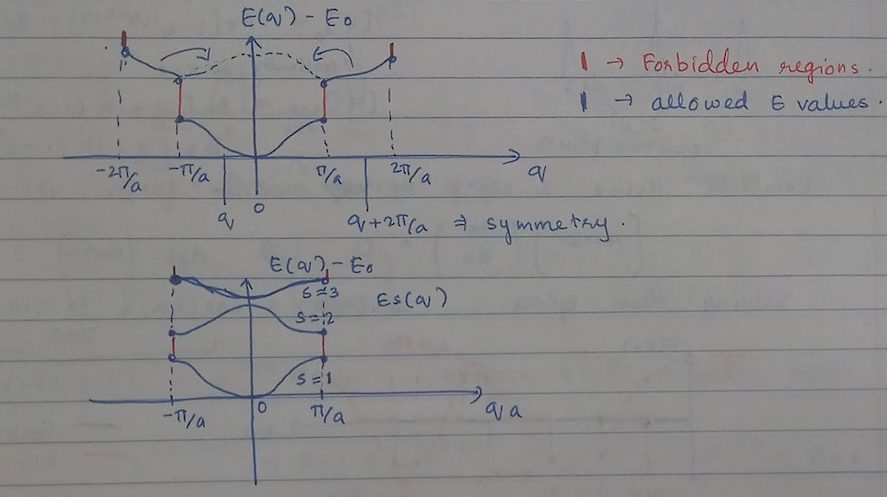
\includegraphics[width=\textwidth/2]{figures/lec_32_band.png}
        \caption{Band Structure for Dirac Comb}
        \label{fig:band_structure_for_dirac_comb}
    \end{figure}
\end{ex}

\end{document}
